In this chapter we compare a choice of game development \textit{systems} and \textit{programming languages}. We start by giving a background on systems and languages, and we compare the two according to their general advantages and disadvantages. We discuss the pragmatic reasons behind the adoption, by most developers, of systems instead of languages. We then discuss in more detail some notable game development systems, and we choose three of them for their significance and current adoption. We do the same for programming languages, that is we pick three of them that we deem particularly relevant for comparison and inspiration. From our survey and our previous discussions, we conclude that there is a need for more exploration of specialized languages for game development, as these can give significant advantages that are currently not exploited by game developers.


\section{Systems vs languages}
A game development system is a collection of libraries and tools that are used to build games. A game development system mainly features pre-built functionality that the developer instances in those places where he needs them. For example, by using an editor, the developer may drag the functionality for moving something around with mouse and keyboard onto a model, which then becomes controllable with the user input. Game development systems often feature some customizability by supporting user-defined scripts. Such scripts are small programs that modify limited aspects of the game, for example the formulas that compute the damage of specific weapons, custom triggers and timers, etc. Scripts do not modify the core services of the system. Some game development systems are mostly focused on libraries, which are then accessed through a programming language. Pre-built functionality is then leveraged by invoking the library functions or instancing the library data-types. Such libraries are accompanied by tool support, for example custom project settings for popular development environments.

A game development language is a programming language that is used to build games. A game development language mainly features syntactic constructs that directly map to abstract aspects of the game. For example, a game development system may have a specialized syntax to support drawing the game world or reading the user input. A game development language focuses on a new expressive paradigm rather than leveraging existing knowledge or using intuitive interfaces.

Systems and languages are the two ends of the continuum of software development. Software development represents a continuum because some development systems may feature custom programming languages for limited scripting, or new programming languages may feature exotic editors to accompany them. Despite this continuum, the main philosophies behind systems and languages differ significantly. Systems tend to be conservative towards developer effort, in that they try to reduce the amount of notions that the developer has to express in order to build the game by reducing the amount of code written, and by allowing the exploration of functionality through visual interfaces. Languages, on the other hand, focus on how the developer approaches the problem, and are design to offer the maximum possible expressive power by reducing obvious or repetitive code.

Both systems and languages offer advantages over one another, and both have some disadvantages. In general, systems represent a safe investment where we leverage high-quality components built by others, while taking advantage of existing technical knowledge to the fullest. Systems often have limitations in their expressive power. These limitations come in many forms. It may be that all games built from a system are similar in some manner, or that specific, advanced tasks cannot be changed at all or at least easily. Language, on the other hand, represent a risky investment where we spend a lot of learning effort in order to gain new abilities on how to express the various solutions to the issues encountered while building games. These abilities empower the developer to build games quicker, with less mistakes, and with clearer and simper code. Languages for making games do not trade expressive power for simplicity, but are harder to learn because of their novel approaches.

Systems are safer to use, and as such most companies use game development systems rather than game development languages. The rise of many high-quality commercial game development systems in the last decades means that there are lots of available game development systems of proven worth. Game development languages, on the other hand, have not been developed much outside the academia, and even in it there are only few significant efforts in this direction. Commercial adoption of game development languages, thereby, is insignificant.


\section{Systems for making games}

A discussion of all existing game-development systems is beyond the scope of this work, as it could be the subject of an entire thesis all by itself. Existing game-development systems cover a large variety of game scenarios: there exist multiple engines for first person shooters, multiple engines for role-playing games, multiple engines for flight simulators, and so on for many genres of games and simulations. This happens because games represent an interactive virtual reality. Virtual reality is any simulation that flows in real-time with its rules, its logic, its goals, and its means of interaction. Such a virtual reality may be similar to actual reality in some aspects, but it may also depart from realism significantly. The number of ways that a virtual reality may be designed is large: any aspect, from physics, to rendering, to the introduction of fantasy elements and interaction schemes may be changed at will. This implies that there is a large space of possible games, with an important consequence: for many games it can be difficult to find existing systems that fully meet their creative needs, and sometimes an existing system that seems to meet the initial specification may fail to accommodate the evolving needs of the game, because the designers may decide half-way during development to add some new features that are not well supported by the system. This situation arises from the fact that game development systems only support \textit{specific} scenarios in terms of the type of games they can build. There exist systems that support first-person-shooter games with a focus on physics and high-quality rendering of few characters in smaller environments, systems that allow rendering a racing track with cars running at very high speeds (the physics and rendering of high-velocity entities offer a challenge all of their own), systems that focus on rendering few characters at a time in third-person for role-playing-games, systems that focus on rendering large armies that clash in large-scale strategic battles, and many others. In the following, we list some game development systems that are relevant either because of historical reasons, or because of their widespread adoption. We then pick three relevant systems for further study.


\subsection{Relevant game systems}
There are many other game development systems and engines. The earliest examples of game engines built for use in multiple games include several 2D game creation systems built in the 1980s. Among these, Pinball Construction Set \cite{CHAPTER_3_PINBALL_CONSTRUCTION_SET}, Adventure Construction Set \cite{CHAPTER_3_ADVENTURE_CONSTRUCTION_SET}, Garry Kitchen's GameMaker \cite{CHAPTER_3_GARRY_KITCHENS_GAME_MAKER}, Wargame Construction Set \cite{CHAPTER_3_WARGAME_CONSTRUCTION_SET}, Shoot'Em-Up Construction Kit \cite{CHAPTER_3_SHOOT_EM_UP_CONSTRUCTION_KIT}, Arcade Game Construction Kit \cite{CHAPTER_3_ARCADE_GAME_CONSTRUCTION_KIT}, and most popularly ASCII's RPG Maker engines which are still being released at regular intervals \cite{CHAPTER_3_RPG_MAKER}.
The 1990s saw the first generation of graphics engines: BRender from Argonaut Software \cite{CHAPTER_3_BRENDER}, Renderware from Criterion Software Limited \cite{CHAPTER_3_RENDERWARE}, and RenderMorphics' Reality Lab \cite{CHAPTER_3_REALITY_LAB} (which eventually turned into Direct3D \cite{CHAPTER_3_REALITY_LAB_INTO_DIRECT3D}).

The term "game engine" was adopted starting from the mid-1990s, especially in connection with FPS games. In particular, the Doom and Quake games were so popular that other developers licensed portions of those games code in order to build their own games by just designing the games content (levels, graphics, etc.). Later incarnations of games were designed with this approach in mind, to the point that games such as Quake III arena and Unreal (and their successors) were built with the goal of licensing their engines \cite{CHAPTER_3_ID_TECH, CHAPTER_3_UNREAL_ENGINES}. Game engines were adopted in other genres; for example, the Gamebryo engine \cite{CHAPTER_3_GAMEBRYO} was used both in the Morrowind and Dark Age of Camelot RPG games.

The short list of systems just presented only covers some game-genres, but there are many other genres such as adventure games, platformers, flight simulators, etc., all with their own systems and engines that solve their specific requirements. In short, most existing systems do not accommodate all possible game designs, since they are built with a specific boundary in supported games. Games that are not supported by existing systems either need new systems or they need heavy modifications of existing systems in order to fulfill their special needs.

Among the most notable systems we also find lower level frameworks such as DirectX \cite{CHAPTER_2_DIRECT3D_10} or OpenGL \cite{CHAPTER_2_OPENGL}, which simply offer a set of libraries plus some additional tools such as debuggers or profilers, to be used from existing programming languages and IDEs.


\subsection{Our choice of systems}
Three interesting representatives of the current trends: \textit{(i)} \textit{Game Maker} \cite{CHAPTER_2_GAME_MAKER} is a game development system which focuses on the simple philosophy of "less is more", and by doing so it allows even complete beginners to be able to make articulated games. Game Maker is a visual environment that limits the user to 2D games based on "rooms" with 2D sprites representing objects, characters, etc. interacting in them; \textit{(ii)} \textit{Unity} \cite{CHAPTER_2_UNITY}, on the other hand, is a powerful and flexible game development tool which offers the possibility of building 3D games in a visual environment; with a system of generic components that can be activated on each entity to make it respond to physics, input, etc., it allows to express many different scenarios; we will also discuss \textit{(iii)} \textit{XNA} \cite{CHAPTER_2_XNA}, a modern framework that is oriented to coding indie games and which supports many common tasks of game development with .Net languages such as C\#, VB .Net, and F\#.

The systems we consider are chosen to represent both game engines and game libraries. We deem them particularly relevant because they are widely adopted among indie game developers, serious game developers, and even in educational circles. We exclude engines such as UDK and Quake, not because of their quality (which is extremely high), but because they are applied to specific game development tasks (AAA games) which are not those this thesis focuses upon (indie and serious games).


\subsection{Game Maker}
GameMaker is an IDE that allows users to easily develop computer games without the requirement of prior computer programming experience, while also allowing advanced users to create complex applications with its built-in scripting language.

GameMaker's primary development interface is based on a drag-and-drop system. The available menus allow the creation and organization of a hierarchical structure of sprites which represent the rooms where the game takes place and the entities that will inhabit the game world. Available icons represent the most common actions that are interesting in a game, such as movement, basic drawing, and simple control-flow idioms that allow the definition of reactions such as collision detection.

Since dragging and dropping may allow the definition of simple games but is limiting when advanced users wish to express things like AI, pathfinding, etc., GameMaker contains a built-in scripting programming language called the \textit{Game Maker Language} (GML). GML can access and modify most of the game entities values, it can perform loops, and in general is a fully fledged programming language. GML is interpreted, with its interpreter being embedded in stand-alone GameMaker games.

GameMaker primarily uses 2D graphics, with all the additional functionality expected beyond simple drawing of sprites, such as alpha adjustments and blending settings. In latest versions GameMaker started supporting more advanced graphics functions, among which a limited ability to use 3D graphics.  Note that this feature is intended exclusively for the most advanced users of GameMaker.

Game Maker can be seen in action in Figure \ref{fig:game_maker_in_action}.

\begin{figure}
\begin{center}
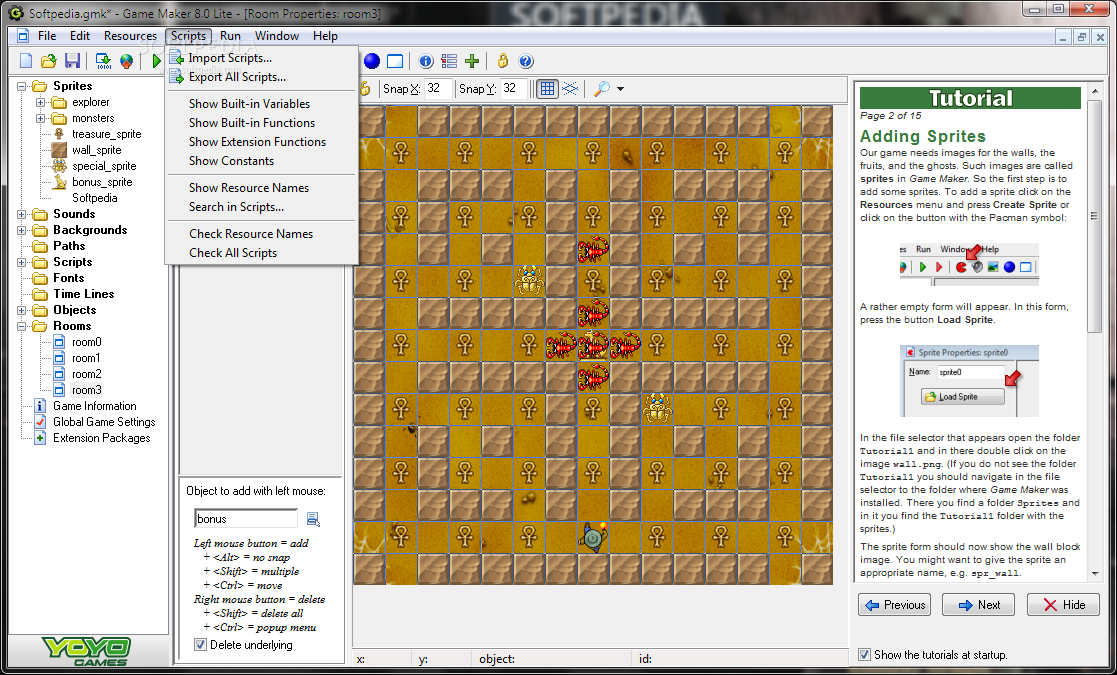
\includegraphics[width=8cm]{Pics/gamemaker1.png}
\end{center}
\caption{Game Maker in action}
\label{fig:game_maker_in_action}
\end{figure}

\subsubsection{Unity 3D}
Unity 3D is an asset-centric game-development system. This means that Unity tries to keep the game developer as much as possible into the visual editor, dragging new game objects into the scene hierarchy, modifying the game objects properties to customize their appearance or behavior along certain predefined ways. The editor also maintains a live preview of the game. Unity 3D supports high quality 3D rendering through support of normal maps, shadows, full-screen post processing, and more.

The underlying architecture is based on components. Components are properties of a game entity that allow a certain entity to follow certain rules. Components may be the ability to follow physics rules, to respond to input commands, and so on. When the developer selects an entity in the editor, he then attaches components to the entity so that it will perform the desired actions.

As in GameMaker, not everything for a moderately complex game can be expressed in a visual editor. Unity supports the execution of custom game scripts via Mono, the open-source implementation of the .NET Framework. Scripts may be written in UnityScript (a custom language inspired by JavaScript), C\#, or the Boo programming language \cite{CHAPTER_3_BOO}.

A screenshot of Unity is shown in Figure \ref{fig:unity_in_action}.

\begin{figure}
\begin{center}
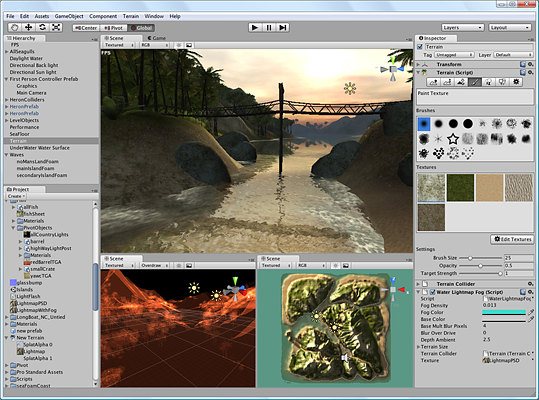
\includegraphics[width=8cm]{Pics/unity1.png}
\end{center}
\caption{Unity in action}
\label{fig:unity_in_action}
\end{figure}

\subsubsection{XNA}
Both GameMaker and Unity pragmatically include a scripting system so that game objects can be manipulated with user-written scripts. These scripts track some logical aspects of the game state, such as score, lives, re-spawning, AIs, etc., and may either be run in response to certain events, or during every tick of the simulation. This may seem in contrast with the visual nature of those editors, which offer many options to create games in a "mostly code-free" fashion. What this ultimately means is that game development is inextricably tied to coding, no matter how powerful visual environments are used. Visual environments can help \textit{reduce} the need to write code, but the number of useful game functions that may be defined is simply so large that expressing it without having to type them in a programming formalism is very hard. For example, consider the number of AI algorithms in existence: state machines, neural networks, fuzzy logic, planning system, genetic algorithms, etc. Furthermore, new algorithms are constantly under study and get published every year. This means that for a game system to support this large amount of algorithms, simply pre-programming all of them is not feasible: they are too many, and new ones are added all the time. 

In short, game development requires coding.

For this reason we also discuss the XNA framework. XNA is a code-centric tool for making games based on the .Net framework. XNA can be used from any .Net language: from C\#, to F\#, to VB.Net. It offers classes that cover most areas of game development. Such classes represent an efficient and easy to use implementation of those small building blocks that are found in virtually all games. XNA starts by supporting the game loop with the \texttt{Game} and \texttt{GameComponent} classes, which manage the creation of the game window, and the invocation of the tick functions of the game loop at the appropriate times. Input is supported by polling the mouse, keyboard, and XBox 360 gamepad. To ease building collision detection and physics, a series of bounding volume classes are supported such as boxes, spheres, planes, etc. that may be checked for intersection with each other. XNA also offers rendering facilities so that the developer can quickly add 2D rendering of alpha-blended sprites and 3D rendering of simple models. Rendering may also use shaders, render targets, and similar advanced features in conjunction with the simple drawing primitives: this makes it possible to create advanced visual effects. Audio is supported with music, positional 3D sounds, and even pre-mixed audio effects created with the XACT audio editor. Networking is, unfortunately, supported only on the XBox with a UDP library that also includes functionality for lobby, friends, invites, and all those features that support some of the more social aspects of multiplayer.

XNA does not offer any visual framework or helper, and instead requires coding all a game, often with a large amount of code.

The XNA "Racing Car Starter Kit" shows the potential of the framework in Figure \ref{fig:xna_in_action}.

\begin{figure}
\begin{center}
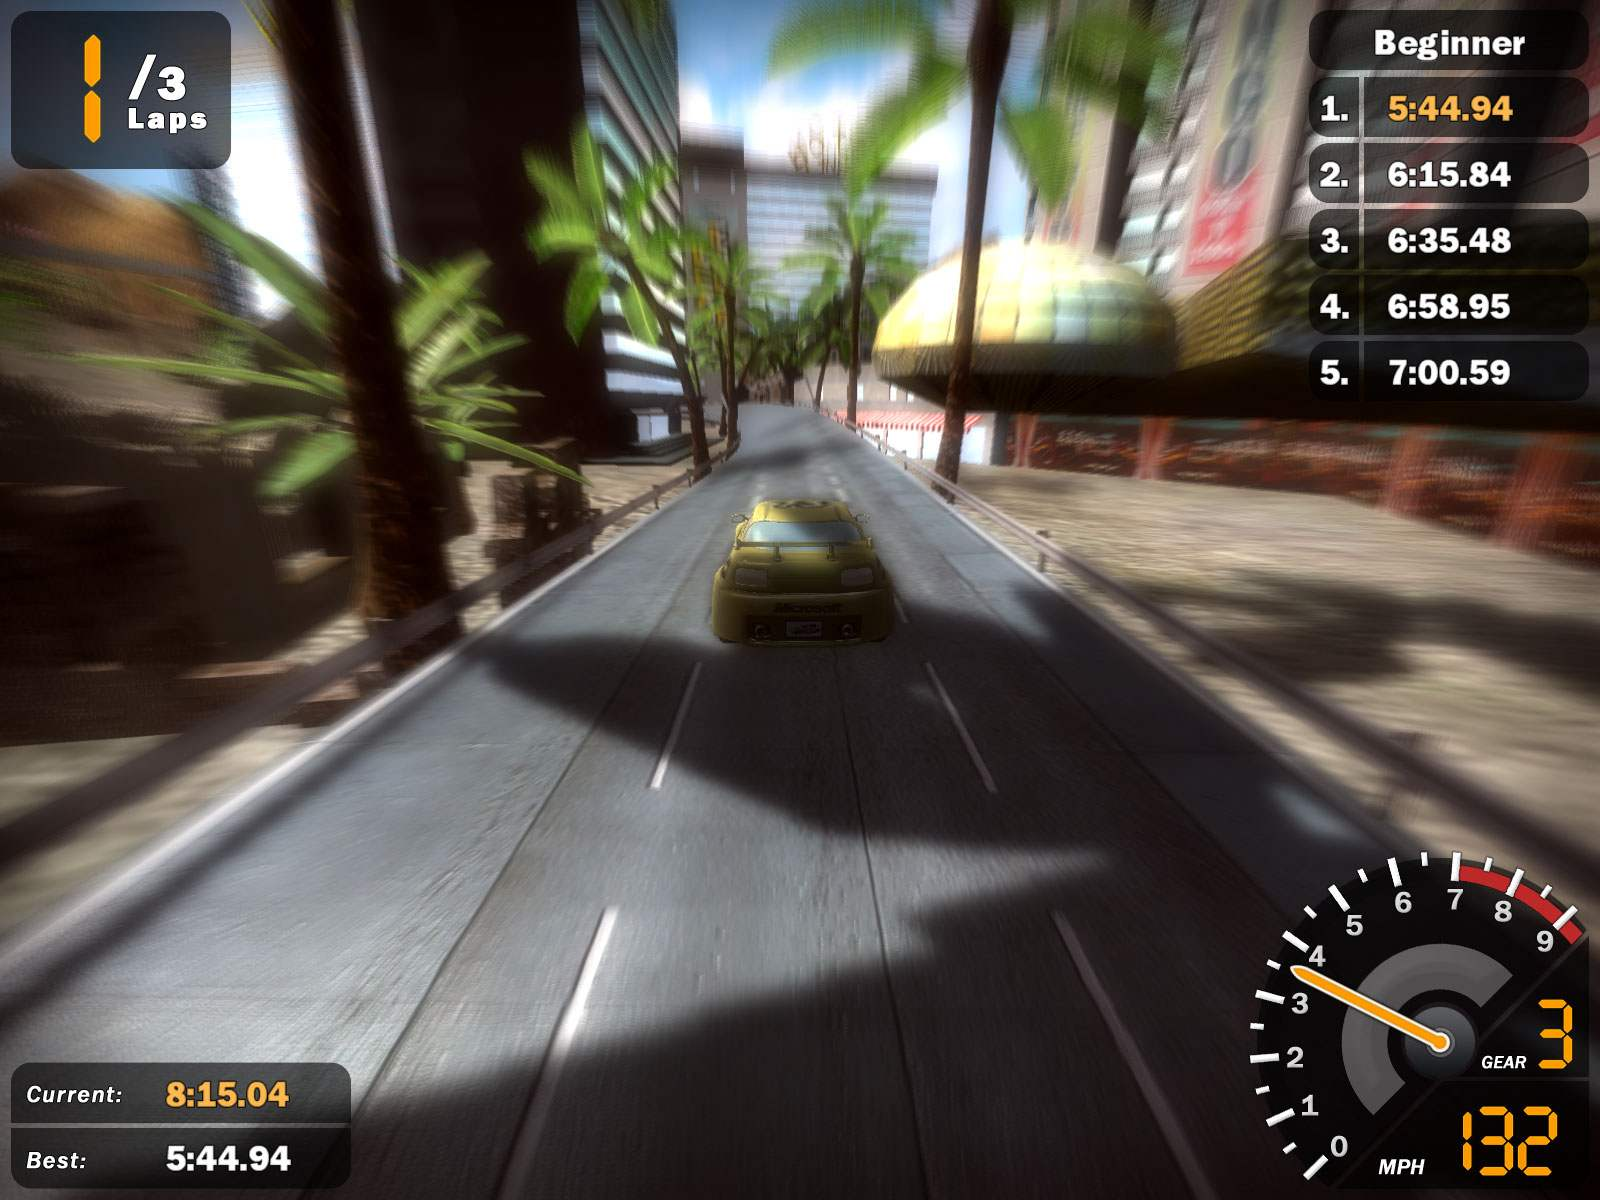
\includegraphics[width=8cm]{Pics/xna1.png}
\end{center}
\caption{XNA in action}
\label{fig:xna_in_action}
\end{figure}


\section{Languages for making games}

Game development can also be done with special-purpose programming languages. Game-development languages are not many, and the possible reasons are multiple: \textit{(i)} building a language is complex and requires specialized knowledge about compilers, parsers, and type-systems, all in addition to knowledge in the specific domain (in our case games) to which the language applies; \textit{(ii)} game development systems compensate their lack of expressive power through the integration of scripting languages; \textit{(iii)} the game development industry is very slow to adopt new programming languages when compared to the IT industry in general, and this has resulted in a very slow progression in the last decades from assembly to C and finally to C++; this is partly due to huge existing code-bases of C/C++ code that is still being used in production, and from the fact that a shift in language would require extensive retraining.

Outside the gaming industry some researchers have experimented with building languages for making games, while the industry mostly focused on libraries for C, C++ or, in later years, C\# as well. The languages built by researchers have all focused on specific aspects of game development, resulting in a very diverse, albeit slightly small, set of specialized languages. The game-specific languages that we will discuss in the following of this chapter are: \textit{(i)} \textit{Simula} \cite{CHAPTER_2_SIMULA67}, an old language built for simulations where many innovations in programming languages were born; \textit{(ii)} \textit{SGL} \cite{SGL}, a recent language from Cornell University which unified the definition of a game loop with a series of heavily optimized SQL-style queries on a global table that stores all the game entities; and \textit{(iii)} \textit{Inform 7} \cite{CHAPTER_2_INFORM}, a programming language which only focuses on a small group of games, that of textual adventures, but allows to write them in plain English instead of a traditional, structured and symbolic programming language.

\subsection{Simula 67}
The first language we discuss is the Simula language, in particular the Simula 67 version (there are two versions: Simula I, and Simula 67, the second being more advanced). Simula is quite an old language, and was one of the precursors of modern object-oriented languages. It was born in 1967, and it focused strongly on building simulations, as the name aptly suggests. In particular, Simula featured objects, inheritance, and a notion of cooperative multi-threading through \textit{coroutines}. Simula ships with a simulation package that allows building discrete event simulations. Simula is also a historically relevant language, in that its object system laid the groundwork for the implementation of objects that is now found in languages such as C++, Java, and C\#. Moreover, Simula made heavy use of coroutines, which are now widely used in modern programming languages to define generators to create collections interactively; coroutines are notably making a comeback in the C\# language in the form of the \texttt{async} and \texttt{await} keywords. Moreover, before \texttt{async} and \texttt{await}, Mono and Unity introduced a customized version of coroutines with the \texttt{yield} statement.

Let us now consider an example of the simulation capabilities of Simula. Sam, Sally, and Andy are shopping for clothes. They have to share one fitting room. Each one of them is browsing the store for about 12 minutes and then uses the fitting room exclusively for about three minutes, each following a normal distribution. A simulation of their fitting room experience is as follows:

\begin{lstlisting}
Simulation Begin 
  Class FittingRoom; Begin 
    Ref (Head) door; 
    Boolean inUse; 
    Procedure request; Begin 
      If inUse Then Begin 
        Wait (door); 
        door.First.Out; 
      End; 
      inUse:= True; 
    End; 
    Procedure leave; Begin 
      inUse:= False; 
      Activate door.First; 
    End; 
    door:- New Head; 
  End;

Procedure report (message); Text message; Begin 
  OutFix (Time, 2, 0); OutText (": " & message); OutImage; 
End;

Process Class Person (pname); Text pname; Begin 
  While True Do Begin 
    Hold (Normal (12, 4, u)); 
    report (pname & " is requesting the fitting room"); 
    fittingroom1.request; 
    report (pname & " has entered the fitting room"); 
    Hold (Normal (3, 1, u)); 
    fittingroom1.leave; 
    report (pname & " has left the fitting room"); 
  End; 
End;

Integer u; 
Ref (FittingRoom) fittingRoom1;

fittingRoom1:- New FittingRoom; 
Activate New Person ("Sam"); 
Activate New Person ("Sally"); 
Activate New Person ("Andy"); 
Hold (100); 
End;
\end{lstlisting}

The \texttt{Simulation} keyword at the beginning of the listing enables the use of simulations. The fitting room object uses a queue called \texttt{door} that arbitrates access to it. If someone requests the fitting room while it is in use, then they must wait in the queue with the \texttt{Wait (door)} statement. When the fitting room is emptied, the first person in the queue is activated with \texttt{Activate door.first} and removed from the queue \texttt{door.First.Out}. A person is modeled as a \texttt{Process} and its activity is described using the \texttt{Hold} statement that suspends the process to simulate browsing the store and being in the fitting room. The person process uses the \texttt{request} and \texttt{leave} methods to obtain and release access to the fitting room.

The main program initializes and activates the various entities of the simulation, which is then run for 100 minutes of simulated time before the program terminates.

Simula pioneered the use of many constructs for building simulations. Even today, programming languages have not managed to achieve the same level of expressive power for simulations that Simula programmers enjoyed. The example above, for instance, would be harder to write in a general-purpose programming language such as C++, given the lack of first-class support for cooperative multi-thread, queues, etc.


\subsection{Inform}
The Inform 7 language is the latest incarnation of Inform, a programming language and design system for interactive fiction originally created in 1993 by Graham Nelson. Inform 7 is a peculiar programming language, in that it addresses a "niche-within-a-niche" of the domain of computer programming. Inform exclusively allows the building of interactive text adventure games, that is those kind of games where the game world is presented to the user with a textual description, and the input that the user gives is, again, with textual commands. This makes Inform's scope \textit{extremely} specific.

The most advanced feature of the Inform programming language is that it allows the programmer to write a game in plain English, albeit with certain grammatical limitations. The language allows the description of the game as a series of objects with properties, together with a series of scenes that the user interacts with. The parsing facilities offered by Inform are indeed very powerful, and they are used to parse the user's input and the programmer's code both expressed in natural language. Inform features a simple object system that allows only for single inheritance and polymorphism; the language is also statically and strongly typed, in order to allow the programmer to reuse some code, but without adding complex notions such as abstraction, so that the concepts that come into play are always as simple as possible. This means that some traditional programming activities are supported by the language, but all constructs are declarative and highly readable.

A sample Inform 7 program could be:

\begin{lstlisting}
"Hello Deductible" by "I.F. Author"

The story headline is "An Interactive Example".

The Living Room is a room. "A comfortably furnished living room." The Kitchen is north of the Living Room. The Front Door is south of the Living Room. The Front Door is a door. The Front Door is closed and locked.

The insurance salesman is a man in the Living Room. "An insurance salesman in a tacky polyester suit. He seems eager to speak to you." Understand "man" as the insurance salesman.

A briefcase is carried by the insurance salesman. The description is "A slightly worn, black briefcase." Understand "case" as the briefcase.

The insurance paperwork is in the briefcase. The description is "Page after page of small legalese." Understand "papers" or "documents" or "forms" as the paperwork.

Instead of listening to the insurance salesman for the first time:

say "The salesman bores you with a discussion of life insurance policies. From his briefcase he pulls some paperwork which he hands to you."; move the insurance paperwork to the player.
\end{lstlisting}

Inform does not feature many of the constructs that would be necessary to build a complex, real-time simulation: there is no notion of a main loop, nor is the language designed to define real-time actions or describe rendering methods besides text. From the point of view of making games \textit{in general} it is woefully under-powered, but when it comes to interactive fiction it is, quite literally, a unique experience to use.

Multiple games have been built with Inform. \textit{Curses}, by Graham Nelson, was the first game ever written in the Inform programming language. \textit{So Far}, by Andrew Plotkin, won the first XYZZY Award for Best Game winner in 1996. \textit{Galatea}, by Emily Short, is considered to have the most complex interaction systems for a non-player character in an interactive fiction game. \textit{Mystery House Possessed}, again by Emily Short, was the first Inform 7 game released to be public. Emily Short's \textit{Floatpoint} won the Interactive Fiction Competition, and the 2006 XYZZY awards for Best Setting and Best NPCs.


\subsection{SGL}
The final language we discuss is the SGL language. SGL, as the name suggests, is a language that descends from the widely known SQL language for expressing declarative queries on databases. 

SGL is based on the idea of defining the game world as a large table of entities, where an entity is a row with a union of all the attributes possible for all entities; all the attributes that are irrelevant to a specific entity are then set to null values. The dynamics of the game, such as physics, damage, grouping, etc. are then defined in terms of a huge query that transforms all entities from one time-step of the simulation into another.

For example, an SGL game could define a unit in a virtual army as:

\begin{lstlisting}
class Unit {
  State:
    number unit_id;
    number player;
    number command;
    number pos_x, pos_y;
    number health;
    Set<number> squad;
  Effects:
    number move_x : AVG;
    number move_y : AVG;
    number damage : SUM;
    Set<number> joined : UNION;
    Set<number> left : UNION;
  Update:
    pos_x = pos_x + move_x;
    pos_y = pos_y + move_y;
    squad = squad UNION joined SETMINUS left;
    health = health - damage;
}	
\end{lstlisting}

The \textit{state} encodes a description of the entity with a set of attributes. The \textit{effects} define a series of queries (similar to Casanova rules) that are further specified as described below. The \textit{update} specifies how the state of the entity changes at every tick of the game loop.

Queries that move units towards enemy clusters may be defined with SQL-style aggregations such as:

\begin{lstlisting}
let enemies = (all u in Units where u.player != me.player);
let centroid_x = AVG(enemies.x_pos);
let centroid_y = AVG(enemies.y_pos);
let me.move_x = (me.pos_x - closest.pos_x)/norm;
let me.move_y = (me.pos_y - closest.pos_y)/norm;
\end{lstlisting}

SGL games retain most of the readability of SQL queries, that is, even though an SGL game will not be as simple and pleasant to read as an Inform code listing (few programming languages can boast such feature), it is still far simpler to read than equivalent low-level code. The high-level semantics at which SGL games are expressed allows the SGL engine to know more about what computations the game performs; SGL, for example, will be able to understand that we wish to compute a certain Cartesian product between certain lists, and it will be able to automatically create a support index to turn the evaluation of this product from the $O(n^2)$ complexity of the naïve implementation into the much lower $O(n \log n)$ of a balanced search tree. The complex algorithmic optimizations made by SGL are usually done by hand in traditional game development (often many times in the same game) by developers, and with lots of effort. In this sense SGL allows a developer to create a game without worrying about performance but obtaining the run-time performance that results from the use of hand-written, specialized, complex algorithms.

SGL also assumes the presence of other game engine modules such as a rendering module, an input module, and even pathfinding facilities. From this point of view SGL is not a fully-fledged game programming language, but it allows building efficiently the core module of a modern game.


\section{Motivating a new programming language}
Creating a new programming language may be seen as a fruitless endeavor. Specifically, there are many programming languages that have been created as part of research efforts. Very rarely such languages have seen widespread adoption, and virtually all of them have been confined to research labs.

It should be noticed that the purpose of such research has never been that of creating industrial-grade tools that are used by many. Rather, the purpose of programming languages research is to shed new light on the best practices by exploring \textit{unknown possibilities} \cite{CHAPTER_1_PL_RESEARCH}. Indeed, many defunct research languages actually paved the way for innovations in future languages \cite{CHAPTER_1_PL_INFLUENCE_ON_PL} and even tools and systems that are now wide-spread (for a recent example, see \cite{CHAPTER_1_PL_INFLUENCE_ON_CURRENT_LANGUAGES}). Also, programming language research has often automated lessons from the field of Software Engineering, as described in \cite{CHAPTER_1_PL_AND_SWENG}.
Sometimes there have even been decades of difference in terms of time between invention and adoption. One need only realize that research in programming languages has yielded benefits that range from sub-routines \cite{CHAPTER_1_PL_SUBROUTINES}, to data structures \cite{CHAPTER_1_PL_DATASTRUCTURES}, to objects \cite{CHAPTER_1_PL_OBJECTS}, to delegates and callbacks \cite{CHAPTER_1_PL_HOF}, to generics \cite{CHAPTER_1_PL_INFLUENCE_ON_PL}, to compile-time meta-programming \cite{CHAPTER_1_PL_GENERIC_PROGRAMMING}, to garbage collection \cite{CHAPTER_1_PL_GARBAGE_COLLECTION}, and so on.

The motivation for choosing to create a programming language rather than trying to engineer (yet another) game development system, is also grounded in the observation that there exist many game development systems. From top-of-the-line game engines such as ID's engines, CryTek, Aurora, etc. to simpler tools aimed at hobbyist or indie developers such as Unity, GameMaker, XNA, and others, most existing systems either fall short in generality (it is rare that an FPS engine works well for other genres, such as RTSes, and vice-versa), they fall short in expressive power, or the do not offer a significant advantage to developer besides a few handy facilities.

Additionally, as game development tools and systems are a heavily explored field, we argue that designing a language for making games is a welcome departure from traditional approaches, and it may lead to novel insights and understanding in the field.

it is a possible source of novel insight to study how the problem of game development can be tackled by language design.

In general, building a programming language offers relevant advantages over designing a system. Ever since the dawn of computer science, programming languages have flourished. Despite Church and Turing's insights that all programming languages are born equal, new programming languages keep on being invented, each with its own strengths and weaknesses. 

In the following we explore some of the strengths afforded to programming language designers. We do not claim that the list of items discussed below is complete, nor do we claim that it is our own invention and discovery. What follows is distilled from a survey of the literature, with particular focus on seminal works such as \cite{CHAPTER_1_PL_OBJECTS, CHAPTER_1_CODE_MANAGEMENT, CHAPTER_1_PL_INFLUENCE_ON_PL, CHAPTER_1_PL_TYPE_SYSTEMS_AND_MEMORY_ALIGNMENT, CHAPTER_1_PL_AND_SWENG, CHAPTER_1_TESTING_DOES_NOT_WORK}, as highlighted by our our own experience. From this, we observe that languages are primarily: \textit{(i)} syntactic abstraction mechanisms that reduce repetitive code; \textit{(ii)} thought shapers that induce a paradigm shift in how one should structure software; \textit{(iii)} simplifiers that boil down an existing paradigm to just its essential parts, often to increase understanding and insight; \textit{(iv)} law enforcers that make sure important invariants hold, to increase correctness, performance, or other properties. 

We now discuss how a programming language affects the \textit{(i)} flexibility, \textit{(ii)}  correctness, and \textit{(iii)} efficiency of the programs written in it. We describe why and how each of these three aspects is important for games and briefly note the relevance of each item with respect to game-development. We also explain how game development systems and languages fare in that regard.

\subsection{Flexibility}
Software is flexible when it is \textit{easy to understand, modify, and extend}. This is achieved through structuring the program well, but a programming language can help with the structuring.

Games are modified and tuned up to the very end of their development cycle, and sometimes even beyond \cite{CHAPTER_1_PATCHING_CYCLES}. This means that flexible architectures for making games are of importance for game developers.

Game development systems are usually designed with a series of predefined scenarios in mind, and depending on the system it may well be impossible to push it beyond its originally intended boundaries, even if it is sometimes needed. This makes such systems not truly flexible.

Flexibility depends on abstraction \cite{CHAPTER_1_CODE_MANAGEMENT,CHAPTER_1_PL_INFLUENCE_ON_PL}, which allows to reuse code and define general solutions that can be reused across similar problems that arise multiple times.

\subsubsection{Abstraction}
The ability to create hierarchies of libraries makes it possible for a developer to capitalize on the work done by others before him. Programming languages allow the definition of \textit{reusable units}: procedures and functions allow avoiding duplicating code, data abstraction allows to reuse "similar" but otherwise different data-types in the same context without rewriting the same operation many times, and entire modules can be abstracted with design patterns.

Games feature huge code bases \cite{CHAPTER_1_SIZE_OF_GAMES} that we argue could be greatly reduced in size if some forms of abstraction were used to avoid re-writing large similar parts. Game engines are a relevant example of this process in action.

Abstraction is impossible (or much harder to achieve) with systems where the user only has a GUI to perform actions. This happens because even though action sequences can be recorded, it is hard to make the recorded sequence \textit{parametric} so that with a simple change in some parameter then we obtain a different (but similar) sequence of actions.

\subsection{Correctness}
Software is always supposed to achieve a certain task under certain \textit{requirements of correctness}. Programming languages can help establish certain degrees of correctness by offering ways to specify and check important properties \cite{CHAPTER_1_PL_STATIC_ANALYSIS}.

In game development, correctness constraints could be specified so that, for example, the language ensures the correct dimensional analysis for physics quantities, the correct generation of state machines, etc.

Systems that are well-designed and well-tested often offer strong correctness guarantees, since they force the user to interact with the project only according to a predefined set of rules and by sanitizing his input so that only safe operations are performed.

Correctness depends on: \textit{(i)} memory safety to ensure that the program does not manipulate nonsensical values; \textit{(ii)} concurrency control to arbitrate accesses to shared resources; and \textit{(iii)} testing to find bugs, or exclude them to a certain degree.

\subsubsection{Memory Safety}
Accessing unallocated memory, jumping to data-addresses, or in general \textit{carelessly manipulating memory addresses} can result in catastrophic, hard to debug errors. By using a static type-system that ensures that all data manipulated and passed to procedures is of the correct type ensures that memory accesses are always properly aligned \cite{CHAPTER_1_PL_TYPE_SYSTEMS_AND_MEMORY_ALIGNMENT}. Static type systems have no run-time overhead, that is after the program is type-checked at compile time the produced assembly code has no trace of the types used during compilation. Garbage collection also helps ensuring such safety \cite{CHAPTER_1_PL_GARBAGE_COLLECTION}.

Games manage large numbers of objects with unpredictable, highly dynamic lifetimes. This makes a reliable memory system useful because thanks to it the developer does not have to manually track the life-cycle of an entity to deallocate its representation by hand; such a technique risks to maintain references to a deallocated entity, or to not deallocate some entities that are not references anymore and which thus occupy memory for no reason.

Game systems achieve correctness through extensive testing \cite{CHAPTER_1_PATCHING_CYCLES}, and often make use of unsafe memory manipulation techniques \cite{CHAPTER_1_POINTER_ARITHMETICS_IN_GAME}. As such, they only offer empirical guarantees (through extensive testing \cite{CHAPTER_1_TESTING_DOES_NOT_WORK}) about the memory safety of games, and moreover they never exclude the possibility of memory leaks or similar mishaps since running the game may encounter conditions which did not occur during testing.

\subsubsection{Concurrency Control}
Languages often operate on shared resources accessed by \textit{concurrent processes}.

This is particularly relevant in a game, where many entities operate concurrently on the game world \cite{CHAPTER_1_GAMES_ARE_CONCURRENT}, and they must be synchronized in order to guarantee that the logical invariants of the game are respected.

A system can have a predefined, monolithic system for managing concurrency, while a language can define a paradigm that (to various degrees) arbitrates access to shared resources \cite{CHAPTER_1_PL_AND_RESOURCE_SHARING}.

\subsubsection{Bug finding}
Most software development is spent on \textit{testing}, rather than writing code \cite{CHAPTER_1_TESTING_MORE_THAN_WRITING}. By forcing certain properties on a program (or on parts of it), such as the absence of side-effects in functions, it becomes easier to test a program in a bottom-up fashion. The absence of side-effects allows testing smaller pieces of the program in isolation first, and then testing their composition until most of the program is tested properly. In contrast, programs where many functions read and write on lots of global values requires testing one's program against all combinations of function call sequences and initial values of the shared state: such a task may be nigh impossible.

The number of possible configurations in a game world is very large, given that many entities in the game can move, change their internal statistics, etc. The very large space that must be tested in games allows them to benefit significantly from a bottom-up testing strategy in the absence of side effects, since this would reduce the number of tests to be performed while being assured that composing the smaller parts of the game that have been tested preserves correctness.

Game systems usually allow the definition and concurrent manipulation of global game variables, and in general suffer the issue where the insertion in the game of an apparently innocent and (locally) correct procedure may suddenly break something else (which may even appear to be unrelated).

\subsection{Efficiency}
Software efficiency is measured by the amount of resources it uses to accomplish its task. A variety of resources can be considered, from time and space to network bandwidth, power, and databases. When \textit{resources are constrained}, a language' constructs and compiler can be made aware of these resources and even of the possible optimization strategies \cite{CHAPTER_1_COMPILER_OPTIMIZATIONS}. A language can make it easier to express efficient algorithms by supporting efficient data structure declaration and traversal; for example, we can observe that building a balanced binary tree is simpler \footnote{Or at least much closer to its definition in mathematical notation, and relatively far from the technical details of a computer.} to do with union types (see Appendix \ref{chap:fsharp}) in the style of ML rather than with C structures and pointers. A compiler or interpreter such as those used for SQL can also heavily elaborate the input program and insert the appropriate optimizations so that the user does not have to do so by hand (and sometimes without even being aware of them) and still get an efficient program \cite{DATABASE_SYSTEM_IMPLEMENTATION}.

In game development CPU time is a crucial resource, since if the game runs slowly then the gaming experience will fail to be immersive and the game will have missed its mark. A language that is aware of the needs of a game can help by ensuring that any code written for the game will be optimized automatically, for example running certain portions of the game logic in parallel or optimizing Cartesian products with the use of spatial partitioning indices.

Game development systems usually provide a series of commonly used underlying services such as rendering, input management, and physics, which are highly optimized; they then rely on the game developer to not write code that will slow down the game excessively.


\section{Creating new languages for making games}
As a conclusion, we note that game development, even with the most advanced systems, still requires a significant amount of programming. Unfortunately, this is not done with special-purpose programming languages; such languages would yield significant benefits (as discussed in the previous section) to game developers, and such benefits are currently ignored completely by game development companies. Moreover, game development systems have shortcomings which are often just worked around by game developers, as outlined in the comparison of Table \ref{tab:systems vs languages}. Therefore, from the next chapter on we will introduce the Casanova language, designed exclusively for making games. Our objective is not that of designing and building \textit{the} ultimate game development language. Our aim is less ambitious: we will simply show the benefits of adopting \textit{a} game development language, as long as it is properly designed.

\begin{table} 
\center
\begin{tabular}{ | p{7cm} | p{7cm} |}

\hline
Systems & Languages \\
\hline

easier to use from the start & harder to use from the start \\ & \\

leverage existing technical knowledge & obtain new knowledge \\ & \\

write small amounts of code & write large amounts of code \\ & \\

leverage high quality components done by others & leverage high quality components done by others \\ & \\

obtain good results with little effort right away & obtain good results with little effort after the learning phase \\ & \\

games from a system look similar to one another & games can vary a lot between one another \\ & \\

expressive power is limited & expressive power is absolute \\ & \\

complex tasks that are not pre-built have no support or even awkward support & all complex tasks are supported \\

\hline

\end{tabular}
\caption{Systems vs languages}
\label{tab:systems vs languages}
\end{table}


\begin{comment}
One aspect that emerges from the analysis of game development systems and languages is that coding is an ubiquitous activity that cannot be marginalized or outright removed from game development. Nevertheless, smartly designed visual editors that access well-written libraries can save a good deal of development effort by allowing the developer to drag-and-drop to place objects and activate their properties; after this phase, scripts of code are written as needed, to realize more complex behaviors that are not supported by the underlying libraries. This means that even the best designed systems can benefit from powerful languages for game development. We argue that the use of game development languages that are built for general-purpose use is inappropriate, since the features of these languages often are incompatible with the needs of the game.

We believe that one final detail is worthy of notice. All visual editors require, at some point, the use of a programming language to express some of the most complex custom aspects of a game. This means that their difficulty curve is at most as high as that of their languages, even if novices that do not (yet) write code for their game may not notice it in the beginning, thus giving the impression of an easier to use system. As such, visual editors simply postpone as much as they can the difficulties of learning how to program for games, and they automate some common game programming activities, but they do not eliminate the need for coding.
\end{comment}
